\documentclass[a4paper,11pt]{article}

\usepackage[utf8]{inputenc}
\usepackage[margin=1in]{geometry}
\usepackage[T1]{fontenc}
\usepackage{lmodern}
\usepackage{amsmath, amssymb, amsthm}
\usepackage{graphicx}
\usepackage{hyperref}
\usepackage{geometry}
\usepackage{listing}
\usepackage{color}
\setlength{\parindent}{0pt}
\setlength{\parskip}{1em}
\usepackage{booktabs}
\usepackage{caption}
\usepackage[ruled,vlined]{algorithm2e}
\usepackage{subcaption}
\usepackage{bookmark}
\usepackage[
    backend=biber,
    style=authoryear,
  ]{biblatex}


\addbibresource{bibliography.bib}

\title{BART: A Comparison with Non-bayesian Tree Methods}
\author{
    Vincenzo Dorrello 
    \and
    Giulio Frey 
    \and
    Guido Rossetti 
    \and
    Giovanni Scarpato 
}
\date{\today}

\begin{document}

\maketitle

\begin{abstract}
Your abstract here.
\end{abstract}

%\tableofcontents

\section{Introduction}
summary of all
\cite{chipmanBARTBayesianAdditive2010}

\section{Decision trees}
CART (Classification And Regression Trees) trees, where first introduced by (\cite{Breiman et al. 1984}) and represent a statistical method for constructing decision trees for both regression and classification problems. 
A CART is an upside-down tree, in the sense that leaves are at the bottom of the tree. Terminal nodes, that is nodes without descendants, are called leaves, whereas the other nodes are called internal nodes. Each internal node has two child nodes, hence the tree is said to be binary. The segments of the trees that connect the nodes are called branches. The internal nodes are labeled by a condition while the leaves by a value of the dependent variable. Hence, when a tree is given, is easy to do forecasting. Indeed, to get the predicted value $\hat{y}$  for a given covariate vector $x$, is enough to go sequentially answer the decision rules starting form the root of the tree. For each decision rule, if the condition of is verified you go to one side of the node, if not, you go to the other. This process continues until the terminal node is reached. The set of bottom nodes (or leaves) of the trees give a partition of the space of covariates: it partitions the space of covariates $x$ into $J$ distinct non-overlapping regions $R_1, \ldots, R_J$, each corresponding to a terminal node of the tree. 

Regression trees are very different models compared with the more common linear regression models.  Suppose there are $n$ observations of $y$ and $\mathbf{x} = (x_1, \ldots, x_p)$. Overall, covariates and output are related by the equation
\begin{equation}
    Y = f(X) + \epsilon, \quad \epsilon \sim \mathcal{N}(0, \sigma^2), \label{regression}
\end{equation}
where we assumed normality of the error for simplicity.
Both regression trees and linear models attempt at making inference about the unknown function \( f \), which is left completely unrestricted, using the \( p \)-dimensional vector of inputs \( x = (x_1, \dots, x_p) \) and the output $y$. 
How $f(X)$ is proxied depends on the model chosen. On the one hand, linear regression models assume a functional form of the type:
\begin{equation}
  f(X) = \beta_0 + \sum_{j=1}^p X_j \beta_j
\end{equation}
On the other hand, regression trees approximate the function $f(X)$ with a step-wise form: 
\begin{equation}
  f(X) = \sum_{j=1}^J \mu_j \cdot 1(X \in R_j) \label{stepwise}
\end{equation}

where $R_1, ..., R_J$ represent the partition of the covariates space generated by the leaves of the tree.
The preferable method depends on the particular problem we are presented with. Indeed, if the relation among explanatory variables and the dependent variable is well approximated by a linear model, it is likely that a linear regression will outperform a regression tree model. On the contrary, if there is a highly non-linear and complex relation between the explanatory variables and the dependent one, then a regression tree is more likely to outperform a simple linear regression model. Moreover, when fitting a regression tree instead of a linear model, we do not have to care about the scale of covariates.
From now on our analyses will only focus on models of the form of \eqref{stepwise}.

We take most of our arguments for this section from the \cite[Chapter~8]{jamesIntroductionStatisticalLearning2021}, and from \cite{Random Forest with R}.

\subsection{Regression Trees}
 
Regression trees are built in two steps.
First, the predictor space (the set of all possible values of the vector of observables $X_1, ...., X_p$) is split into $J$ regions $R_j$ that are distinct and non-overlapping.  Secondly, given a new observation $x$ that falls in a region $R_j$, the model predicts the corresponding outcome variable $\hat{y}$ to be the mean of the outcome variables corresponding to the observations in the training set that fall in that same region.

To begin, we have to construct the regions $R_1,..., R_j$. For simplicity, regions are chosen as $p$-dimensional boxes, where $p$ is the number of regressors. The partition is chosen is such a way to minimize the RSS:  
\begin{equation}
  \{R_1,...,R_J \}=\operatorname*{argmin}_{ \{R_j\}_{j=1}^J}\sum^J_{j=1}\sum_{i\in R_j}\left(y_i-\hat{y}_{R_j}\right)^2
  \label{rss_tree}
\end{equation}
where $\hat{y}_{R_j}$ is the mean of the training observation in the $j$-th box.

It is computatioanlly infeasible to do the optimization problem in \eqref{rss_tree}. Instead of considering all the possible partitions of the predictor space, a top-down, greedy approach, known as recursive binary splitting is used. The approach is \texttt{top-down} since it begins at the top of the tree, and then sequentially splits the predictor space; each split is then indicated by two new branches. Moreover, the process is \textit{greedy}, since for each step we make that split that generates the greatest reduction of the RSS at that particular step, and we do not choose the best sequence of steps looking ahead.
\\To perform recursive binary splitting, the algorithm considers the set of all predictors $X_1, \ldots, X_p$, and the set of all possible values of the cutpoint $s$, and then choose the predictor $X_j$ and the cutpoint $s$ such that the branching of the tree corresponding tot the decision rule:  $$\{X \mid X_j < s\} \quad \text{and} \quad \{X \mid X_j \geq s\}$$ minimizes the RSS. Then, we repeat the process within the resulting subregion, looking again for the predictor and the cutpoint such that the subsequent decision rule minimize the RSS. It is important to note that this time we do not split the entire predictor space but one of the two previously identified regions. This process continues until a stopping condition is reached; the more common requires a minimum number of observation within each splitting nodes.

\subsection{Pruning}

Recursive binary splitting to build a regression tree  is likely to produce good prediction on the training-set but overfit the training data, leading to poor out-of-sample performance.The reason is that the above mentioned procedure is likely to give us a complex tree, which has probably a low bias but high variance in prediction. Constraining ex ante the size of trees would be a short-sighted solution, because one could possibly stop too soon, leaving potentially good splits further down in tree unachieved.
\\A better strategy is pruning an already complex tree. This amounts to search for a good intermediate between two extreme cases: a fully developed tree which has high variance but low bias, and a tree consisting of only the root, with high bias but low variance. 
The strategy consists in growing a very large tree $T_0$, and then prune it back in order to obtain a subtree. To do so, we use cost complexity pruning, also know as weakest link pruning.

Consider a sequence of subtrees of $T_0$, $\{T\}_\alpha$ indexed by a non-negative tuning parameter $\alpha$.
For each value of $\alpha$, there is a subtree $T \subset T_0$ such that
$$\sum_{m=1}^{|T|} \sum_{i : x_i \in R_m} \left( y_i - \hat{y}_{R_m} \right)^2 + \alpha |T|$$
is as small as possible, where $|T|$ represents the number of terminal nodes of the tree T, $R_m$ is the subset of the predictor space corresponding to the $m$-th terminal node, $\hat{y}_{R_m}$ is the predicted response associated with $R_m$.
The tuning parameter $\alpha$ controls the trade-off between a sub-tree complexity and and its fit to the training data, the higher the $\alpha$, the more terminal nodes a tree has, the smaller a subtree is.
The value for $\alpha$ can be chosen using a validation set or trough cross-validation.

\subsection{Pros and Cons of decision trees}
Overall, CART offers much greater flexibility in handling the relation between covariates and output than linear models do. This comes from the fact that fitting a regression tree amounts to estimate a stepwise relation between $y$ and the covariates $x$ that can proxy well non-linear patterns. 
Greater flexibility of CART comes in handy also when dealing with missing values. CART offers an effective way to overcome this issue, by constructing surrogate variables. Exploiting correlation between predictors, CART may decrease the effect of missing data. 

So far we considered only binary splits, thus an interesting question would be if a model with more than two splits at each note is a valid idea. However, it turns out that in general is not a good strategy. The issue is that multiple splits fragment the dataset too quickly. Moreover, since multiple splits can be achieved by a series of binary splits, the latter approach is preferred.

The interpretability of CART trees has been one of the driving forces of its success. Indeed, thanks to its structure, is straightforward to understand why, for a given $x$, we expect a particular value of $y$, following a series of decision rules. Small trees are visually easy to interpret. Moreover, trees build in such a way are a computationally fast method, that easily scales with large datasets.

However, one of the main disadvantages of this setting, is that trees are non-robust. In fact a small change in the data can lead to a large change in the estimation. This follows from the fact that regression trees suffer from high variance. The main reason of this instability is the hierarchical structure of the process as the effect of an error in one of the first nodes is propagated to the other nodes below it. This is heightened by the fact that single trees tend to overfit, and spurious correlations in the training data can be mistaken as structural patterns and included in the decision rules. This may lead to bad out-of-sample predictive performance. High variance and tendence to overfit are the main reasons that simple regression trees are not used by practitioners. Instead, ensemble methods are generally preferred. 

\section{Ensemble methods}

An ensemble method is an approach that aims at combining many ensemble methods that combine the fit from many (hundreds, thousands) simpler models to get an overall
 predictor. These simpler models are often called weak learners, since often lead to mediocre prediction if considered singularly.
All the models we are going to discuss, namely Bagging, Boosting, Random Forest and Bayesian Additive Regression Trees are ensemble methods, for which the simpler models consist of regression trees.

\subsection{Bagging}
Bagging, or Bootstrap Aggregation, is a general method that aims at reducing the variance of a statistical learning method. The method is based on the fact that, given independent observations, averaging over them reduces the variance.
For the case of regression trees, we would like to be able to take many different training sets from the population, to build a different trees for each training set and then to average the resulting predictions. However this is very unfeasible since we do not have access to many training sets. Hence, we resort to bootstrap. 
Bootstrapping consists of taking repeated samples, with replacement, from the single available training set. In such a way, we are able to construct $B$ different bootstrapped training sets.

Bagging consists in taking $B$ bootstrap samples from the training data, each of the same size as the training data, and to fit a large tree to each bootstrap sample. Then it combines the results from each of the $B$ trees to get an overall prediction.
The single predictions for the target funciton $f(X)$ for each sample are averaged, as
\begin{equation}
  \label{eq_bagging}
  \hat{f}_{\text{bag}}(x) = \frac{1}{B} \sum_{b=1}^{B} \hat{f}^{*b}(x).
\end{equation}
where $B$ is the number of samples of the bootstrapping procedure.

In bagging the trees are grown big and are not pruned. Therefore, each single tree has high variance and low bias. Averaging these different trees reduce the variance. 

The drawback of bagging is that we lose interpretability to improve accuracy. When we bag a large number of trees, we can no longer represent the model with a single tree.

\subsection{Random Forest}
A possible problem with bagging is due to the lack of randomization between trees. Indeed, since trees are separately fitted on the bootstrapped training set, it may happen that they share to great amount the same decision rule. This is the case, for example, if there is very strong predictor in the dataset. Hence, in the collection of bagged trees a vast majority of the trees will use this strong predictor in the top split and tehy will all be hihgly correlated among themselves.
\\Correlation among the trees in turn decrease the effectiveness of averaging, as it does not lead to a large reduction in variance, making the entire bagging algorithm less useful. 
 Random Forests starts from bagging and adds another kind of randomization to reduce correlation among trees. Rather than searching over all the covariate space for each decision rule, as the greedy build of the big trees imposes, in random forests we randomly sample a subset of $m$ covariates to search over each time we make a split. Therefore, the split is allowed to consider only one of those m predictors. Moreover, at each split is considered a new sample of m predictors. This makes the big trees explore more the space of models
Usually, we choose $m \approx \sqrt{p}$.
On average, $(p - m)/ = p$ of the splits will not even consider the strong predictor, and so other predictors will have more of a chance. Therefore, we can think of this process as decorrelating the trees, making the average of the resulting trees less variable and hence more reliable.


\subsection{Boosting}

Differently from bagging and random forests, boosting does not involve fitting independent trees from many bootstrap samples; instead, boosting relies on fitting trees sequentially, that is, using information from previously grown trees. 
This is shown algorithm \ref{alg_boosting} shows. 
\begin{algorithm} [h]
  \caption{Boosting for Regression Trees}
  \label{alg_boosting}
  \SetAlgoLined
  \DontPrintSemicolon
  \SetKwInOut{Input}{Input}\SetKwInOut{Output}{Output}
  
  Set $\hat{f}(x) = 0$ and $r_i = y_i$ for all $i$ in the training set.\;
  \For{$b = 1, 2, \ldots, B$}{
      (a) Fit a tree $f^b$ with $d$ splits ($d+1$ terminal nodes) to the training data $(X, r)$.\;
      (b) Update $\hat{f}$ by adding in a shrunken version of the new tree:
      \begin{equation}
      \hat{f}(x) \gets \hat{f}(x) + \lambda f^b(x).
      \end{equation}\;
      (c) Update the residuals:
      \begin{equation}
      r_i \gets r_i - \lambda f^b(x_i).
      \end{equation}\;
  }
  Output the boosted model:
  \begin{equation}
  \hat{f}(x) = \sum_{b=1}^B \lambda f^b(x).
  \end{equation}\;
  
\end{algorithm}

By fitting sequentially new trees on the residual of the previous tree, voosting improves at each iteration the fit marginally. Indeed, since there is a constraining parameter $\lambda$, each tree is rather small, with just a few terminal nodes. By 
fitting small trees to the residuals, we slowly improve $\hat{f}$ in areas where it
does not perform well. It is important to mention that in boosting, unlike in bagging, the construction of each tree strongly depends on the trees that have already grown.
The model accounts for three different tuning parameters. The number of of trees $B$, chosen trough cross-validation.  Interestingly, unlike bagging and random forests, boosting can suffer of overfitting if $B$ is too large.
The shrinkage parameter $\lambda$, a small positive number. Common values for $\lambda$ are 0.01 or 0.001, depending on the problem at hand. However, very small values of $\lambda$ often require a very large B to achieve good performances. Lastly, $d$ represents the number of splits in each tree. Often $d=1$ works well. However in this case the tree is called stump since it contains only a single split.




















\section{Bayesian additive regression trees (BART)}
The idea for Bayesian Additive Regression Trees (BART) was first developed by Chipman, George, McCulloch (2010 AOAS). Like other ensemble methods (bagging, boosting, random forest), to solve this regression problem \eqref{regression}, BART approximates \( f(x) = \mathbb{E}(y \mid x) \) by a sum of $m$ regression trees \( h(x) \equiv \sum_{j=1}^m g(x, T_j, M_j)\), where each \( g \) is a regression tree function that given a tree $\theta_j$ to each observation $x$  assigns a leaf $\mu_{ij}$ of that regression tree.
The BART Ensemble Model is therefore
\[
y = \sum_{j=1}^m g(x; T_j, M_j) + \epsilon, \quad \epsilon \sim N(0, \sigma^2) \tag{3}
\]
where for each binary regression tree \( T_j \) and its associated terminal node parameters \( M_j \), \( g(x; T_j, M_j) \) is the function which assigns \( \mu_{ij} \in M_j \) to \( x \). Under \((3)\), \( \mathbb{E}(y \mid x) \) equals the sum of all the terminal node \( \mu_{ij} \)'s assigned to \( x \) by the \( g(x; T_j, M_j) \)'s.
Like the other ensemble methods, to avoid overfitting each tree of the summation must be made a weak learner, explaining only part of the result. To do so, while boosting uses a shrinkage parameter $\lambda$, BART uses a regularization prior:
\[
p((T_1, M_1), (T_2, M_2), \ldots, (T_m, M_m), \sigma)
\]
The prior is set in a way to regularize the fit by keeping the individual tree effects small. It forces each tree to explain only a limited subset of the relationships between the covariates and the predictor variable (it is a marginal addition to the overall fit). By weakening the \( g_j \) effects, BART ends up with a sum of trees, each of which explains a small and different portion of \( f \).


In effect, the \( g_j \)'s become a dimensionally adaptive random basis of weak learners. Bayesian Nonparametrics: Lots of parameters (to make model flexible).
A strong prior to shrink towards simple structure (regularization). BART shrinks towards additive models with some interaction:Fit becomes the cumulative effort of many weak learners.Note that BART works with an ensemble of trees where each tree has an unknown size. As a result, the model is high and random dimensional.  Note that The number of trees $m$ can be much larger than the sample size $n$. Indeed, $g(x; T_1, M_1), g(x; T_2, M_2), \ldots, g(x; T_m, M_m)$ is a highly redundant \textit{over-complete basis} with many parameters.
Finally, dynamic Random Basis Elements:
\[
g(x; T_1, M_1), \ldots, g(x; T_m, M_m) \text{ are dimensionally adaptive.}
\]
It is a highly redundant “over-complete basis” with many many parameters.


Finally, we use MCMC to get draws from the high-dimensional posterior so that  we can stochastically search the model space and gauge our uncertainty. To fit the sum-of-trees model, BART uses a tailored version of Bayesian backfitting MCMC \cite{hastie2000} that iteratively constructs and fits successive residuals.  Inferences obtained from BART are based on successive iterations of the backfitting algorithm, which are effectively an MCMC sample from the induced posterior over the sum-of-trees model space. A single posterior mean estimate of \( f(x) = \mathbb{E}(Y \mid x) \) at any input value is obtained by a simple average of these successive sum-of-trees model draws evaluated at \( x \). Further, pointwise uncertainty intervals for \( f(x) \) are easily obtained from the corresponding quantiles of the sample of draws.


Overall, Bart's characteristics are in how it weakens the individual trees by instead using a prior, and how it performs the iterative fitting by instead using Bayesian backfitting on a fixed number of trees. 
Conceptually, BART can be viewed as a Bayesian nonparametric approach that fits a parameter-rich model using a strongly influential prior distribution. Overall, BART is a highly-dimensional (each tree has unknown size) nonlinear model inspired by boosting and tree ensembles. the main difference is that, being Bayesian, it uses a regularization prior to shrink towards a simple model. It uses MCMC to get draws from the high dimensional posterior so that one can stochastically search the  model space and gauge the uncertainty.

\subsection{The BART Model}
The BART model consists of two parts: a sum-of-trees model and a regularization prior on the parameters of that model.

\subsubsection{A Sum-of-Trees Model}
Denote by \( T \) the tree structure, consisting of a set of interior node decision rules and a set of $b$ terminal nodes. The decision rules are binary splits of the predictor space of the form \( \{x \in A\} \) vs \( \{x \notin A\} \), where \( A \) is a subset of the range of \( x \). We only consider rules based on the single components of \( x = (x_1, \dots, x_p) \) and of the form \( \{x_i \leq c\} \) vs \( \{x_i > c\} \) for continuous \( x_i \). Let \( M = \{\mu_1, \mu_2, \dots, \mu_b\} \) denote a set of parameter values associated with each of the \( b \) terminal nodes of \( T \). Given the way it is constructed, the tree is a full binary tree, that is, each node has exactly zero or two children. 
 Let \( g(x; T, M) \) denote the regression tree function which assigns a \( \mu_i \in M \) to \( x \).
Each \( x \) value is associated with a single terminal node of \( T \) by the sequence of decision rules from top to bottom, and is then assigned the \( \mu_i \) value associated with this terminal node. 
We denote by \( T \) the binary tree structure itself—the various binary split decision rules of the form \( \{x_q < c\} \) versus \( \{x_q \geq c\} \), \( c \in \mathbb{R} \). The vector of parameters associated with \( T \), i.e., the collection of terminal node parameters, is denoted by \( M = \{\mu_1, \ldots, \mu_b\} \), where \( b \) is the number of terminal nodes. Defining a regression tree as \( g(x; T, M) \), we can view \( g(x; T, M) \) as a function that assigns the conditional mean \( \mathbb{E}[y \mid x] \) to the parameter \( \mu_i \in M \), i.e., \( \mu_i = g(x; T, M) \rightarrow \mathbb{E}[y \mid x] \) via binary decision rules denoted as \( T \).
Thus,
\begin{equation}
Y = g(x; T, M) + \epsilon, \quad \epsilon \sim N(0, \sigma^2)
\end{equation}
is a single tree model. Under (3), the conditional mean of \( Y \) given \( x \), \( \mathbb{E}(Y \mid x) \), equals the terminal node parameter \( \mu \) assigned by \( g(x \mid T, M) \).
With this notation, the sum-of-trees model can be more explicitly expressed as
\begin{equation}
Y = \sum_{j=1}^m g(x; T_j, M_j) + \epsilon, \quad \epsilon \sim N(0, \sigma^2) \label{likelihood}
\end{equation}
where for each binary regression tree \( T_j \) and its associated terminal node parameters \( M_j \), \( g(x; T_j, M_j) \) is the function which assigns \( \mu_{j} \in M_j \) to \( x \). Under (4), \( \mathbb{E}(Y \mid x) \) equals the sum of all the terminal node \( \mu_{j} \)'s assigned by the \( g(x \mid T_j, M_j) \)'s. When the number of trees \( m > 1 \), each \( g(x; T_j, M_j) \) here is merely a part of \( \mathbb{E}(Y \mid x) \), unlike the single tree model.
We can see that the quantity that is being ``summed'' and eventually allocated to \( \mathbb{E}(y \mid x) \) is not the regression tree or tree structure, but the value that each \( j \)th tree structure assigns to the subject. This is one way to think of a sum of regression trees. It allocates a sum of parameters \( \mu_{j} \) to \( \mathbb{E}[y \mid x] \) of the subject.

A sum-of-trees model is an additive function, a sum of step functions of the individual components of \( x \). With a large number of trees, a sum-of-trees model gains increased representation flexibility which, as we'll see, endows BART with excellent predictive capabilities. This representational flexibility is obtained by rapidly increasing the number of parameters. Indeed, for fixed \( m \), each sum-of-trees model (4) is determined by \( (T_1, M_1), \ldots, (T_m, M_m) \) and \( \sigma \), which includes all the bottom node parameters as well as the tree structures and decision rules. Further, the representational flexibility of each individual tree leads to substantial redundancy across the tree components. Indeed, one can regard \( \{g(x; T_1, M_1), \ldots, g(x; T_m, M_m)\} \) as an "overcomplete basis" in the sense that many different choices of \( (T_1, M_1), \ldots, (T_m, M_m) \) can lead to an identical function \( \sum_{j=1}^m g(x; T_j, M_j) \).

\textbf{Nonlinearity of BART.} From this simple example, we can see how BART handles nonlinearity. Each single regression tree is a simple stepwise function or ANOVA model. When we sum regression trees together, we are actually summing together these ANOVA models or stepwise functions, and as a result, we eventually obtain a more complicated stepwise function that can approximate the nonlinearities in the main effect and multiple-way interactions.



\subsubsection{A regularization prior}
In the examples above, we have taken the trees as a given, including which variables to split on, the splitting values, and the mean parameters at each terminal node. In practice, each \( g(x; T_j, M_j) \) is unknown. We therefore need a prior distributions. 

Hyperparameters of $p$ are set so that both the \(T_j\)'s and the 
\(\mu_{ij}\)'s are likely to be small. Thus, $p$ keeps the contribution of each \(g(x; T_j, M_j)\) small, to 
explain only a small portion of the fit. Bart builds up the fit, by adding up tiny bits of fit.  The prior of BART shrinks the model towards additive models with some interaction.

The BART model specification is completed by imposing a prior over all the parameters of the sum-of-trees model, namely, \( (T_1, M_1), \ldots, (T_m, M_m) \) and \( \sigma \). There exist specifications of this prior that effectively regularize the fit by keeping the individual tree effects from being unduly influential. Without such a regularizing influence, large tree components would overwhelm the rich structure of (3), thereby limiting the advantages of the additive representation both in terms of function approximation and computation.

Chipman et al. proposed a prior formulation in terms of just a few interpretable hyperparameters which govern priors on \( T_j \), \( M_j \), and \( \sigma \). When domain information is not available, the authors recommend using an empirical Bayes approach and calibrating the prior using the observed variation in \( y \). Or at least to obtain a range of plausible values and then perform cross-validation to select from these values.

\textbf{Prior independence and Symmetry}
The prior distribution for \eqref{likelihood} is \( p[(T_1, M_1), \ldots, (T_m, M_m), \sigma] \). n order to simplify the specification of the regularization prior, Chipman assumes that  that \( \{(T_1, M_1), \ldots, (T_m, M_m)\} \) are independent of each other and of  \( \sigma \). Then, the prior distribution can be written as:

\[
p[(T_1, M_1), \ldots, (T_m, M_m), \sigma] = p[(T_1, M_1), \ldots, (T_m, M_m)] \, p(\sigma).
\]

\[
= \left[ \prod_{j=1}^m p(T_j, M_j) \right] \, p(\sigma).
\]

\[
= \left[ \prod_{j=1}^m p(M_j \mid T_j) \, p(T_j) \right] \, p(\sigma).
\]
Consider the following. Given $T_j$, let  \( b_j \)  be the number of bottom nodes in the tree \( T_j \). Then \( M = \{\mu_1, \mu_2, \ldots, \mu_{b_j}\} \) is the vector of terminal node parameters associated with \( T_j \).  We assume that each node parameter \( \mu_{ji} \) is iid of each other. This implies: 
\[
p(M_j \mid T_j) = \prod_{i=1}^{b_j} p(\mu_{ij} \mid T_j) \quad \text{(5)}
\]

where \( \mu_{ij} \in M_j \) where \( \mu_i \sim p(\mu) \), iid.
Finally we can write the prior distribution for \eqref{likelihood} as:
\[
p[(T_1, M_1), \ldots, (T_m, M_m), \sigma]= \left[ \prod_{j=1}^m \left( \prod_{i=1}^{b_j} p(\mu_{ji} \mid T_j) \right) \right] \, p(\sigma) \, p(T_j).
\]
Under the independence assumption, we only need to specify \( p(T_j) \), \( p(\mu_{ij} \mid T_j) \), and \( p(\sigma) \). Note that we want to have each $T$ small, each $\mu$ small,  and a "nice " $\sigma$  (e.g. smaller than the least squares estiamte). Indeed, we refer to $p$ as the regularization prior as it restraints the overall fit. In addition, it keeps the contribution of each $g(x;T_i,M_i)$ model component small.  

\textbf{The $T_j$ prior}
The trees $T_j$ are assumed to be iid, so that it is sufficient to define a single $p(T_j)$. Chipman specifies a process 
 that can be used to fraw a tree from the prior. The \( T_j \) prior, \( p(T_j) \), is specified by three aspects:
\begin{enumerate}
    \item The probability that a node at depth \( d = (0, 1, 2, \ldots) \) is nonterminal, given by:
    \[
    \alpha (1 + d)^\beta \quad \text{with} \quad \alpha \in (0, 1) \quad \text{and} \quad \beta \in [0, \infty).
    \]
    Node depth is defined as the distance from the root. Thus, the root itself has depth 0, its first child node has depth 1, etc. This prior controls the tree depth. For a sum-of-trees model with \( m \) large, we want the regularization prior to keep the individual tree components small. To do that, we usually use \( \alpha = 0.95 \) and \( \beta = 2 \).  This makes nonnull but small tree more likely. Nonetheless,  trees with many terminal nodes can be grown if the data demands it.
    
    \item The distribution on the splitting variable assignments at each interior node. Usually, this is the uniform prior on available variables.
    
    \item The distribution on the splitting rule assignment in each interior node, conditional on the splitting variable. Usually, this is the uniform prior on the discrete set of available splitting values.
\end{enumerate}

\textbf{The \( \mu_{i,j} | T_j \) Prior}
We assumed that $\mu_{ij} | T_j$ are iid. For convenience, we first shift and rescale \( y \) so that the observed transformed values range from \( y_{\text{min}} = -0.5 \) to \( y_{\text{max}} = 0.5 \). Then the  prior chosen is:
\[
\mu_{i,j}| T_j \sim N(0, \sigma_\mu^2)
\]
where the zero mean is justified by the centering.  Note that the normal is a conjugate prior. This will simplify posterior inference via MCMC algorithm.
How do we choose the key parameter \( \sigma_\mu \)?
The key observation is that:

\[
f(x | T_j, M_j) = \mu_1 + \mu_2 + \cdots + \mu_{b_j}, \quad \mu_i \sim N(0, \sigma_\mu^2)
\]

You can also just directly set the standard deviation of \( f(x) \):

\[
f(x) \sim N(0, \sigma_f^2)
\]

which is the same as just setting

\[
\sigma_\mu^2 = \frac{\sigma_f^2}{m}
\]

which gives us:

\[
f(x) | T \sim N(0, m\sigma_\mu^2)
\]

which does not depend on \( T \) or \( x \).

\[
\sigma_\mu = \frac{0.5 k}{\sqrt{m}}.
\]
This prior has the effect of shrinking the tree parameters \( \mu_{i,j} \) toward zero, limiting the effect of the individual tree components by keeping them small. Note that as \( k \) and/or \( m \) are increased, this prior becomes tighter and applies greater shrinkage to the \( \mu_{i,j} \). Chipman et al. (2010) found that a value of \( k \) between 1 and 3 yields good results.

Or (\(^ {17}\)), we use the conjugate normal distribution \(N(\mu, \sigma^2)\), which offers tremendous computational benefits because \(\mu\) can be marginalized out. 

To guide the specification of the hyperparameters \(\mu\) and \(\sigma\), note that \(\mathbb{E}(Y \mid x)\) is the sum of \(m\) \(\mu_j\)'s under the sum-of-trees model, and because the \(\mu_j\)'s are a priori i.i.d., the induced prior on \(\mathbb{E}(Y \mid x)\) is \(N(\mu, \sigma^2)\). Note also that it is highly probable that \(\mathbb{E}(Y \mid x)\) is between \(y_{\text{min}}\) and \(y_{\text{max}}\), the observed minimum and maximum of \(Y\) in the data.

The essence of our strategy is then to choose \(\mu\) and \(\sigma\) so that \(N(\mu, \sigma^2)\) assigns substantial probability to the interval \((y_{\text{min}}, y_{\text{max}})\). This can be conveniently done by choosing \(\mu\) and \(\sigma\) so that:

\[
m \mu - k \sigma / \sqrt{m} = y_{\text{min}} \quad \text{and} \quad m \mu + k \sigma / \sqrt{m} = y_{\text{max}}
\]

for some preselected value of \(k\). For example, \(k = 2\) would yield a 95\% prior probability that \(\mathbb{E}(Y \mid x)\) is in the interval \((y_{\text{min}}, y_{\text{max}})\).

The strategy above uses an aspect of the observed data, namely, \(y_{\text{min}}\) and \(y_{\text{max}}\), to try to ensure that the implicit prior for \(\mathbb{E}(Y \mid x)\) is in the right "ballpark." That is to say, we want it to assign substantial probability to the entire region of plausible values of \(\mathbb{E}(Y \mid x)\) while avoiding overconcentration and overdispersion. We have found that, as long as this goal is met, BART is very robust to changes in the exact specification. Such a data-informed prior approach is especially useful in our problem, where reliable subjective information about \(\mathbb{E}(Y \mid x)\) is likely to be unavailable.

For convenience, we implement our specification strategy by first shifting and rescaling \(Y\) so that the observed transformed \(y\) values range from \(y_{\text{min}} = -0.5\) to \(y_{\text{max}} = 0.5\), and then treating this transformed \(Y\) as our dependent variable. We then simply center the prior for \(\mu_j\) at zero (\(\mu = 0\)) and choose \(\sigma\) so that:

\[
k \sigma / \sqrt{m} = 0.5
\]

for a suitable value of \(k\), yielding:

\[
\mu_{ij} \sim N(0, \sigma^2) \quad \text{where} \quad \sigma = \frac{0.5}{k \sqrt{m}}
\]


\textbf{The \( \sigma \) Prior}
We use the inverse chi-square distribution:

\[
\sigma^2 \sim \nu \lambda \chi^2_\nu
\]

Essentially, we calibrate the prior for the degree of freedom \( \nu \) and scale \( \lambda \) for this purpose using a rough data-based overestimate \( \hat{\sigma} \) of \( \sigma \). Two natural choices for \( \hat{\sigma} \) are:

\begin{itemize}
    \item The naive specification, where \( \hat{\sigma} \) is the sample standard deviation of \( y \).
    \item The linear model specification, where \( \hat{\sigma} \) is the residual standard deviation from a least squares linear regression of \( y \) on the original \( X \).
\end{itemize}

We then pick a value of \( \nu \) between 3 and 10 to get an appropriate shape and a value of \( \lambda \) so that the \( q \)th quantile of the prior on \( \sigma \) is located at \( \hat{\sigma} \), i.e., \( P(\sigma < \hat{\sigma}) = q \). We consider values of \( q \) such as 0.75, 0.90, or 0.99 to center the distribution below \( \hat{\sigma} \).

For automatic use, Chipman et al. (2010) recommend the default setting \( (\nu, q) = (3, 0.90) \). It is not recommended to choose \( \nu < 3 \) because it seems to concentrate too much mass on very small \( \sigma \) values, which leads to overfitting.

The choice of \(m\). A major difference between BART and boosting methods is that, for a fixed number of trees \(m\), BART uses an iterative backfitting algorithm to cycle over and over through the \(m\) trees.
BART involves many parameters to ensure flexibility in modeling. Unlike boosting and random forests, the BART algorithm iteratively updates a fixed set of \(m\) trees. A strong prior is used to shrink the model towards simple structures, effectively regularizing the model and encouraging it to align with additive models that incorporate some level of interaction.

\textbf{the choice of m} Selecting a large \(m\) allows for better estimation of \(\mathbb{E}[Y|x]\) and improved predictive performance. With more trees, the model gains greater approximation flexibility, and the components \(g(x; T_1, M_1), \dots, g(x; T_m, M_m)\) become dimensionally adaptive. 

Conversely, choosing a smaller \(m\) highlights variable importance. In this setting, the fewer trees force the predictors \(x\) to compete for inclusion in the model, as seen in gradient boosting. The overall model fit is achieved through the cumulative effort of many “weak learners.”

\textbf{Likelihood Specification for BART}

BART is a sum-of-trees model, i.e., BART assumes that the label \( y \) for an input \( x \) is generated by an additive combination of \( m \) regression trees. More precisely,
\[
y = \sum_{j=1}^{m} g(x; T_j, M_j) + \epsilon,
\]
where \( \epsilon \sim \mathcal{N}(0, \sigma^2) \) is an independent Gaussian noise term with zero mean and variance \( \sigma^2 \). Hence, the likelihood for a single training instance is:
\[
p(y \mid T_j, M_j, \sigma^2, x) = \mathcal{N}\left(y \mid \sum_{j=1}^{m} g(x; T_j, M_j), \sigma^2\right),
\]
and the likelihood for the entire training dataset is:
\[
p(Y \mid T_j, M_j, \sigma^2, X) = \prod_{n=1}^{N} \mathcal{N}\left(y_n \mid \sum_{j=1}^{m} g(x_n; T_j, M_j), \sigma^2\right).
\]


\subsubsection{Posterior inference}

Given the likelihood and the prior, our goal is to compute the posterior distribution:
\[
p\left( \{T_j, M_j \}_{j=1}^{m}, \sigma^2 \mid Y, X\right) \propto p\left(Y \mid \{ T_j, M_j \}_{j=1}^{m}, \sigma^2, X\right) p\left(\{T_j, M_j \}_{j=1}^{m}, \sigma^2 \mid X\right).
\]
Chipman et al. (2010) proposed a Bayesian backfitting MCMC to sample from the BART posterior. At a high level, the Bayesian backfitting MCMC is a Gibbs sampler that loops through the trees, sampling each tree \( T_j \) and associated parameters \( M_j \) conditioned on \( \sigma^2 \) and the remaining trees and their associated parameters \( T_{(j)}, M_{(j)}  \), and samples \( \sigma^2 \) conditioned on all the trees and parameters \( \{ T_j, M_j \}_{j=1}^{m} \).
Let \( T_j^{(i)}, M_j^{(i)} \), and \( \sigma^{2(i)} \) respectively denote the values of \( T_j, M_j \), and \( \sigma^2 \) at the \( i \)-th MCMC iteration. Sampling \( \sigma^2 \) conditioned on \( \{T_j, M_j \}_{j=1}^{m} \) is straightforward due to conjugacy.
To sample \( T_j, M_j \) conditioned on the other trees \( T_{(j)}, M_{(j)}  \), we first sample $T_j \mid T_{(j)}, M_{(j)}  , \sigma$, and then sample $M_j \mid T_j, T_{(j)}, M_{(j)},  \sigma$.
\\More precisely, we compute the residual:
\[
R_j = Y - \sum_{j \neq i} g(X; T_j, M_j).
\]
Using the residual \( R_j^{(i)} \) as the target, Chipman et al. (2010) sample \( T_j^{(i)} \) by proposing local changes to \( T_j^{(i-1)} \).
Finally, \( M_j \) is sampled from a Gaussian distribution conditioned on \( T_j, T_{(j)}, M_{(j)}  , \sigma^2 \).

\subsection{ A Bayesian Backfitting MCMC Algorithm}
NOTE THAT THE DRAWS ARE NOT IID
Given the observed data \( y \), our Bayesian setup induces a posterior distribution:
\[
p\left(T_1, M_1, \ldots, T_m, M_m, \sigma^2 \mid y\right)
\]
on all the unknowns that determine a sum-of-trees model (4). Although the sheer size of the parameter space precludes exhaustive calculation, the following backfitting MCMC algorithm can be used to sample from this posterior. 

At a general level, our algorithm is a Gibbs sampler. For notational convenience, let \( T_{(-j)} \) be the set of all trees in the sum except \( T_j \), and similarly define \( M_{(-j)} \). Thus, \( T_{(-j)} \) will be a set of \( m - 1 \) trees, and the associated terminal node parameters. 

The Gibbs sampler here entails \( m \) successive draws of \( (T_j, M_j) \) conditionally on \( (T_{(-j)}, M_{(-j)}, \sigma^2, y) \):
\[
p(T_j, M_j \mid T_{(-j)}, M_{(-j)}, \sigma^2, y), \quad j = 1, \ldots, m,
\]
followed by a draw of \( \sigma^2 \) from the full conditional:
\[
p\left(\sigma^2 \mid T_1, \ldots, T_m, M_1, \ldots, M_m, y\right).
\]

Hastie and Tibshirani (2000) considered a similar application of the Gibbs sampler for posterior sampling for additive and generalized additive models with fixed bases and showed how it was a stochastic generalization of the backfitting algorithm for such models. For this reason, we refer to our algorithm as backfitting MCMC.

The draw of \( \sigma^2 \) is simply a draw from an inverse gamma distribution and can be easily obtained by routine methods. More challenging is how to implement the \( m \) draws of \( (T_j, M_j) \). This can be done by taking advantage of the following reductions. First, observe that the conditional distribution:
\[
p\left(T_j, M_j \mid T_{(-j)}, M_{(-j)}, \sigma^2, y\right)
\]
depends on \( (T_{(-j)}, M_{(-j)}, y) \) only through:
\[
R_j = y - \sum_{k \neq j} g(x; T_k, M_k),
\]
the \( n \)-vector of partial residuals based on a fit that excludes the \( j \)-th tree. Thus, the \( m \) draws of \( (T_j, M_j) \) given \( (T_{(-j)}, M_{(-j)}, \sigma^2, y) \) are equivalent to \( m \) draws from:
\[
p(T_j, M_j \mid R_j, \sigma^2), \quad j = 1, \ldots, m.
\]

Now, this is formally equivalent to the posterior of the single tree model:
\[
R_j = g(x; T_j, M_j) + \epsilon,
\]
where \( R_j \) plays the role of the data \( y \). Because we have used a conjugate prior for \( M_j \):
\[
p(T_j \mid R_j, \sigma^2) \propto p(T_j) \int p(R_j \mid M_j, T_j, \sigma^2) p(M_j \mid T_j, \sigma^2) \, dM_j,
\]
this can be obtained in closed form up to a normalizing constant. This allows us to carry out each draw in two successive steps as:
\[
T_j \mid R_j, \sigma^2,
\]
and:
\[
M_j \mid T_j, R_j, \sigma^2.
\]

The draw of \( T_j \) can be obtained using the Metropolis-Hastings (MH) algorithm of CGM98. This algorithm proposes a new tree based on the current tree using one of four moves. The moves and their associated proposal probabilities are as follows: growing a terminal node (0.25), pruning a pair of terminal nodes (0.25), changing a non-terminal rule (0.40), and swapping a rule between parent and child (0.10). By integrating out \( M_j \), we avoid the complexities associated with reversible jumps between continuous spaces of varying dimensions.

Finally, the draw of \( M_j \) is simply a set of independent draws of the terminal node \( \mu_j \)'s from a normal distribution. The draw of \( M_j \) enables the calculation of the subsequent residual \( R_{j+1} \), which is critical for the next draw of \( T_j \). 

We initialize the chain with \( m \) simple single-node trees and then iterate until satisfactory convergence is obtained. At each iteration, each tree may increase or decrease the number of terminal nodes by one or change one or two decision rules. Trees may change, cease to exist, or be created. It is not uncommon for a tree to grow large and then subsequently collapse back down to a single node as the algorithm iterates. 

The sum-of-trees model allows for "fit" to be freely reallocated from one tree to another. Because each move makes only small incremental changes to the fit, the algorithm can be imagined as analogous to sculpting a complex figure by adding and subtracting small dabs of clay.

Compared to the single-tree model MCMC approach of CGM98, our backfitting MCMC algorithm mixes dramatically better. When only single-tree models are considered, the MCMC algorithm tends to quickly gravitate toward a single large tree and then gets stuck in a local neighborhood. In contrast, we have found that restarts of the backfitting MCMC algorithm give remarkably similar results even in difficult problems. Consequently, we run one long chain with BART rather than multiple starts. Although mixing does not appear to be an issue, the recently proposed modifications of Blanchard (2004) and Wu, Tjelmeland, and West (2007) might provide additional benefits.

\section{Comparison}
Various methods which combine a set of tree models, so-called ensemble methods, have attracted much attention. These include boosting \cite{freund1997} \cite{friedman2001}, bagging \cite{breiman1996} and random forests \cite{breiman2001}, each of which use different techniques to fit a linear combination of trees.

Boosting fits a sequence of single trees, using each tree to fit data variation not explained by earlier trees in the sequence. Bagging and random forests use randomization to create a large number of independent trees, and then reduce prediction variance by averaging predictions across the trees.

Yet another approach that results in a linear combination of trees is Bayesian model averaging applied to the posterior arising from a Bayesian single-tree model as in \cite{chipman1998} (hereafter CGM98), \cite{denison1998}, \cite{blanchard2004} and \cite{wu2007}. Such model averaging uses posterior probabilities as weights for averaging the predictions from individual trees.
  
\section{Data Application}

We now move to applications of the theoretical insights derived in the previous sections. Firstly, we will focus on simulated data, and then we will cover an application using real word data on abalones.

\subsection{Simulated data}
We simulate a dataframe with the following generating non-linear function:
\begin{equation}
  y = 2\sin(x)+x+Z \quad Z \sim \mathcal{N}(0,1)
\end{equation}
The dataframe is split in two smaller dataframes to obtain training and testing data.

We first run a single decision tree on the simulated data and we obtain as a result 5 terminal nodes and a 
residual mean deviance of 1.164. 

We now fit a BART model with default parameters:  MCMC have 1100 iterations in total of which 100 are burn-in. We see from figure \ref{plot_sin1} that the BART model is able to fit correctly this non-linear trend.

\begin{figure}
  \centering
  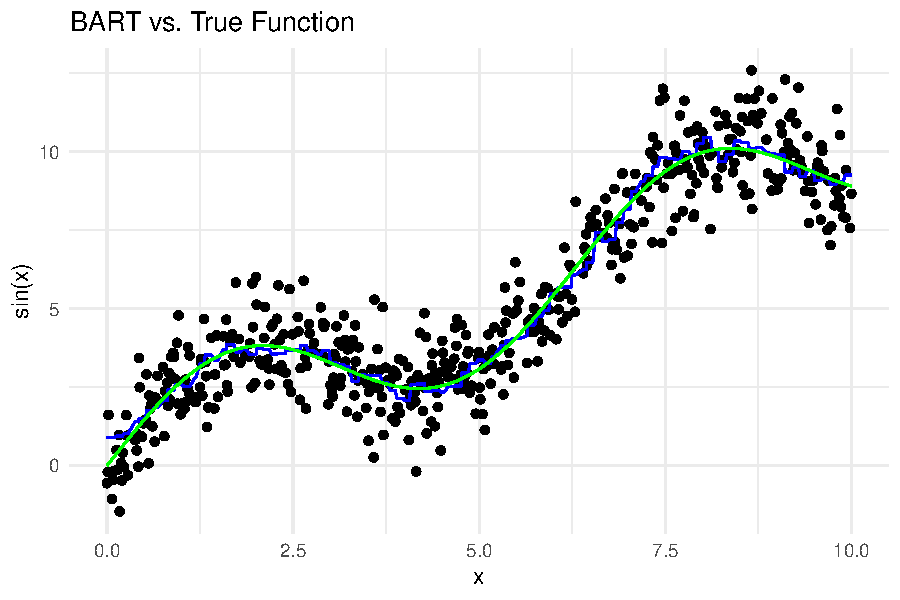
\includegraphics[width=0.7\textwidth]{../outputs/sin_plot.pdf}
  \caption{Plot of the estimates (blue) against observations (black) and generating function(green)}
  \label{plot_sin1}
\end{figure}

To check convergence of the posterior, we plot in figure \ref{plot_sin2} the posterior draws of $\sigma$, the uniquely identified parameter. We observe that the MCMC draw converges quickly to the true parameter, although they oscillate with some autocorrelation due to the posterior sampling procedure.

\begin{figure}
  \centering
  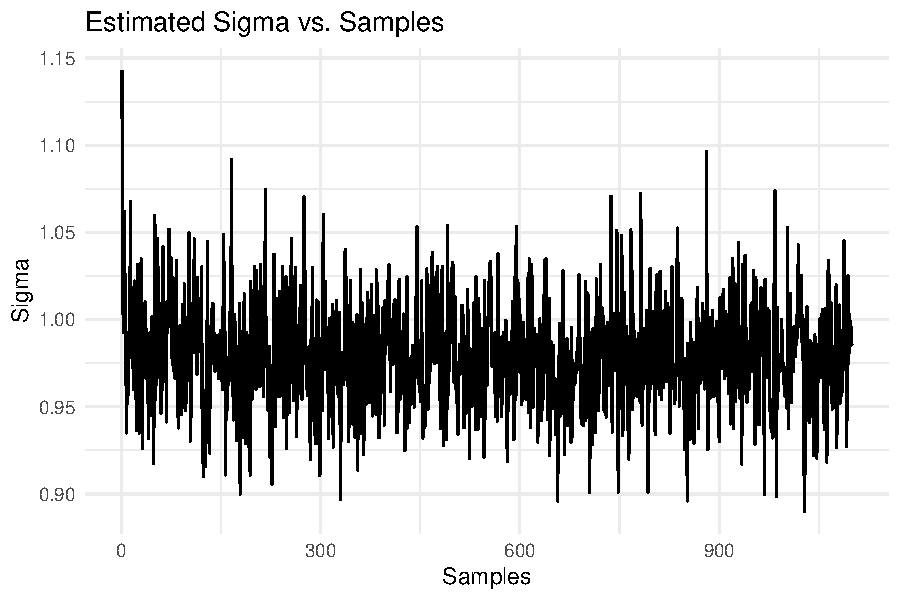
\includegraphics[width=0.7\textwidth]{../outputs/sigma_plot.pdf}
  \caption{Value of $\sigma$ over MCMC iterations}
  \label{plot_sin2}
\end{figure}


To check robustness of BART to different prior specifications, we consider different values for the prior mean of $\sigma$,  that are 100, 0.001 and 1 (the true one). With a large $\sigma$, we observe in plot \ref{plot_sin3} underfitting of the data. With a small $\sigma$, holding all the other parameter constant, the regularization prior is still strong enough to avoid the overfitting.

\begin{figure}
  \centering
  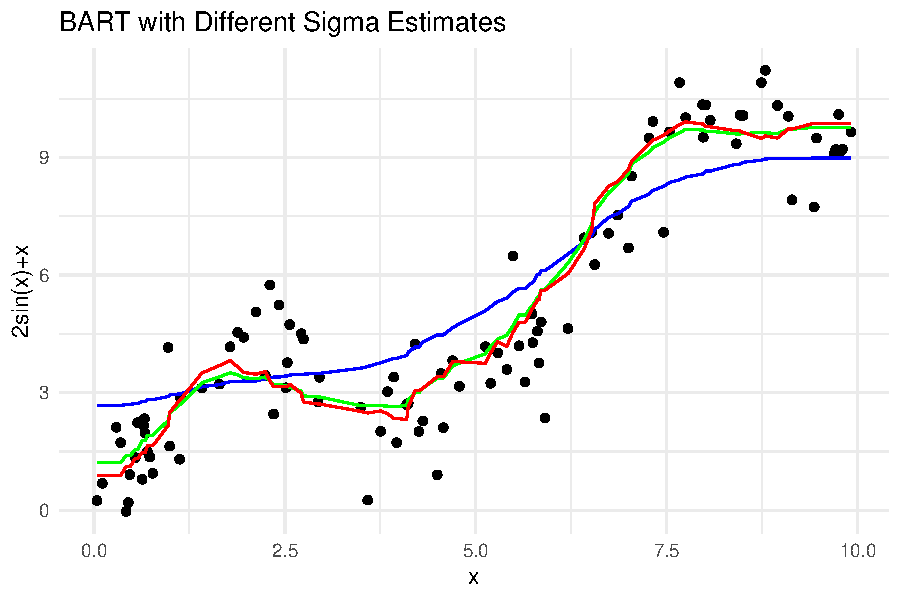
\includegraphics[width=0.7\textwidth]{../outputs/sin_plot_diff_sigma.pdf}
  \caption{DIfferent prior mean of $\sigma$}
  \label{plot_sin3}
\end{figure}


\subsection{Predicting the age of an Abalone}

Abalone are marine snails found in various regions around the world. Determining their age is a labor-intensive process, as it requires cutting through the shell, staining it, and then counting the growth rings under a microscope. However, predicting the age of an abalone can also be done by examining other physical characteristics of the individual, which are much easier to assess. This is precisely the motivation behind our application.

We use data abalone characteristics data coming from the UC Irvine Machine Learning Repository \parencite{warwicknashAbalone1994a}, that is described in table \ref{table1}. No data manipulation is necessary, aside from creating a new variable, \( \text{Age} = \text{Rings} + 1.5 \), and removing the column identifying the number of rings.

\begin{table}[]
  \centering
  \begin{tabular}{llllll}

  \toprule
  Variable Name & Role & Type & Description & Units \\
  \midrule
  Sex                  & Feature       & Categorical   & M, F, and I (infant) & -    \\
  Length               & Feature       & Continuous    & Longest shell measurement & mm\\
  Diameter             & Feature       & Continuous    & Perpendicular to length & mm  \\
  Height               & Feature       & Continuous    & With meat in shell      & mm  \\
  Whole\_weight         & Feature       & Continuous    & Whole abalone           & gram\\
  Shucked\_weight       & Feature       & Continuous    & Weight of meat          & gram\\
  Viscera\_weight       & Feature       & Continuous    & Gut weight (after bleeding) & \\
  Shell\_weight         & Feature       & Continuous    & After being dried       & gram\\
  Rings                & Target        & Integer       & +1.5 gives the age in years & - \\

   \bottomrule
  \end{tabular}
  \caption{Table of Variables}
  \label{table1}
  \end{table}

We run BART from \cite{mccullochBARTBayesianAdditive2024}; Boosting from \cite{ridgewayGbmGeneralizedBoosted2024}; Random Forest and Bagging from \cite{breimanRandomForestBreimanCutlers2024}.Our aim is to compare the predictive performance of those methods. In fact,  we use half of the sample to fit $\hat{y}$, that is the age variable, and half the sample to give us out of bag Mean Squared Errors (MSE) for predicting the same variable. Models are run for various values of T, and for each value, both the mean squared error (MSE) of out-of-sample predictions (shown in plot \ref{plot_mse}) and the computation time (depicted in plot \ref{plot_time}) are recorded.

We observe with a number of trees estimated larger than 500, the BART model is the best performing one, and it reaches also the best performance overall when run with 500 iterations. Although it is the best performer, it is also the model that takes the most to be run, and time of computations scales linearly with the number of trees that are fitted.

\begin{table}[ht]
  \centering
  \begin{tabular}{lcc}
  \toprule
  Model           & MSE & Time (s) \\
  \midrule
  BART            & 4.45    & 66.7  \\
  Random Forest   & 4.53    & 4.74  \\
  Boosting        & 4.87    & 0.220 \\
  Bagging         & 4.54    & 12.4  \\
  \bottomrule
  \end{tabular}
  \caption{Model performance with $T=500$}
  \end{table}


\begin{figure}
  \centering
  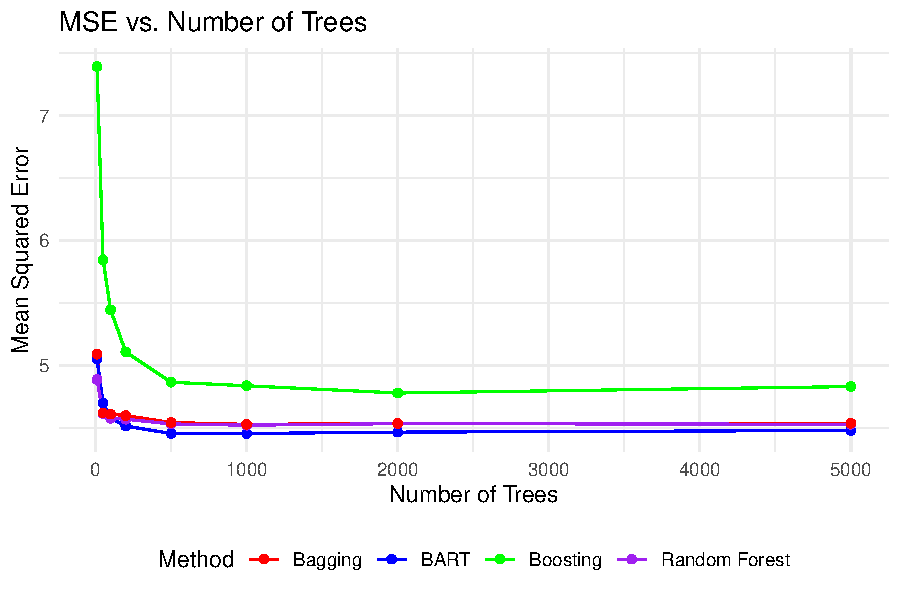
\includegraphics[width=0.7\textwidth]{../outputs/mse_plot.pdf}
  \caption{Mean Squared Error for different values of T}
  \label{plot_mse}
\end{figure}

\begin{figure}
  \centering
  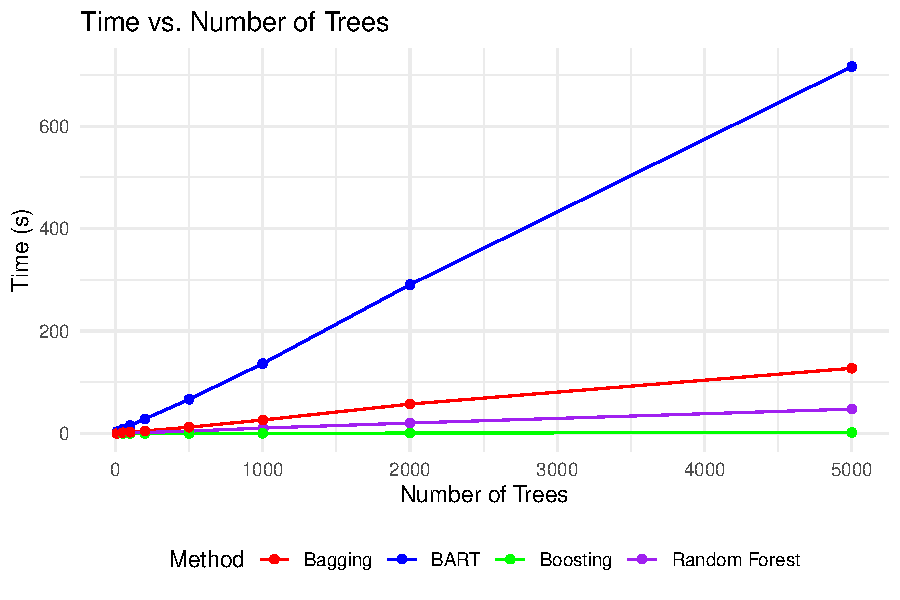
\includegraphics[width=0.7\textwidth]{../outputs/time_plot.pdf}
  \caption{Time of computations for different values of T}
  \label{plot_time}
\end{figure}

\printbibliography

\end{document}